\documentclass[IEEEtran]{IEEEtran}
\usepackage[utf8]{inputenc}
\usepackage{flushend}
\usepackage{listings}
\usepackage{hyperref} 
\usepackage{verbatim} 
\usepackage[pdftex]{graphicx} 
\usepackage[T1]{fontenc}
\usepackage[table]{xcolor}
\usepackage{soul}
\graphicspath{{./images/}}
\urlstyle{same} 

\usepackage{fancyvrb}
\usepackage{color}



\makeatletter
\def\PY@reset{\let\PY@it=\relax \let\PY@bf=\relax%
    \let\PY@ul=\relax \let\PY@tc=\relax%
    \let\PY@bc=\relax \let\PY@ff=\relax}
\def\PY@tok#1{\csname PY@tok@#1\endcsname}
\def\PY@toks#1+{\ifx\relax#1\empty\else%
    \PY@tok{#1}\expandafter\PY@toks\fi}
\def\PY@do#1{\PY@bc{\PY@tc{\PY@ul{%
    \PY@it{\PY@bf{\PY@ff{#1}}}}}}}
\def\PY#1#2{\PY@reset\PY@toks#1+\relax+\PY@do{#2}}

\expandafter\def\csname PY@tok@gu\endcsname{\let\PY@bf=\textbf}
\expandafter\def\csname PY@tok@s2\endcsname{\def\PY@tc##1{\textcolor[rgb]{0.16,0.00,1.00}{##1}}}
\expandafter\def\csname PY@tok@gs\endcsname{\let\PY@bf=\textbf}
\expandafter\def\csname PY@tok@cm\endcsname{\def\PY@tc##1{\textcolor[rgb]{0.25,0.37,0.75}{##1}}}
\expandafter\def\csname PY@tok@gp\endcsname{\let\PY@bf=\textbf}
\expandafter\def\csname PY@tok@m\endcsname{\def\PY@tc##1{\textcolor[rgb]{0.00,0.00,0.00}{##1}}}
\expandafter\def\csname PY@tok@mh\endcsname{\def\PY@tc##1{\textcolor[rgb]{0.00,0.00,0.00}{##1}}}
\expandafter\def\csname PY@tok@ge\endcsname{\let\PY@it=\textit}
\expandafter\def\csname PY@tok@il\endcsname{\def\PY@tc##1{\textcolor[rgb]{0.00,0.00,0.00}{##1}}}
\expandafter\def\csname PY@tok@cs\endcsname{\def\PY@tc##1{\textcolor[rgb]{0.25,0.50,0.37}{##1}}}
\expandafter\def\csname PY@tok@cp\endcsname{\let\PY@it=\textit\def\PY@tc##1{\textcolor[rgb]{0.38,0.38,0.38}{##1}}}
\expandafter\def\csname PY@tok@gh\endcsname{\let\PY@bf=\textbf}
\expandafter\def\csname PY@tok@ni\endcsname{\def\PY@tc##1{\textcolor[rgb]{0.00,0.00,0.00}{##1}}}
\expandafter\def\csname PY@tok@nn\endcsname{\def\PY@tc##1{\textcolor[rgb]{0.00,0.00,0.00}{##1}}}
\expandafter\def\csname PY@tok@na\endcsname{\def\PY@tc##1{\textcolor[rgb]{0.00,0.00,0.00}{##1}}}
\expandafter\def\csname PY@tok@s1\endcsname{\def\PY@tc##1{\textcolor[rgb]{0.16,0.00,1.00}{##1}}}
\expandafter\def\csname PY@tok@nc\endcsname{\def\PY@tc##1{\textcolor[rgb]{0.00,0.00,0.00}{##1}}}
\expandafter\def\csname PY@tok@nd\endcsname{\def\PY@tc##1{\textcolor[rgb]{0.39,0.39,0.39}{##1}}}
\expandafter\def\csname PY@tok@ne\endcsname{\def\PY@tc##1{\textcolor[rgb]{0.00,0.00,0.00}{##1}}}
\expandafter\def\csname PY@tok@nf\endcsname{\def\PY@tc##1{\textcolor[rgb]{0.00,0.00,0.00}{##1}}}
\expandafter\def\csname PY@tok@si\endcsname{\def\PY@tc##1{\textcolor[rgb]{0.16,0.00,1.00}{##1}}}
\expandafter\def\csname PY@tok@sh\endcsname{\def\PY@tc##1{\textcolor[rgb]{0.16,0.00,1.00}{##1}}}
\expandafter\def\csname PY@tok@nt\endcsname{\let\PY@bf=\textbf\def\PY@tc##1{\textcolor[rgb]{0.50,0.00,0.33}{##1}}}
\expandafter\def\csname PY@tok@ow\endcsname{\def\PY@tc##1{\textcolor[rgb]{0.00,0.00,0.00}{##1}}}
\expandafter\def\csname PY@tok@sx\endcsname{\def\PY@tc##1{\textcolor[rgb]{0.16,0.00,1.00}{##1}}}
\expandafter\def\csname PY@tok@c1\endcsname{\def\PY@tc##1{\textcolor[rgb]{0.25,0.50,0.37}{##1}}}
\expandafter\def\csname PY@tok@kc\endcsname{\let\PY@bf=\textbf\def\PY@tc##1{\textcolor[rgb]{0.50,0.00,0.33}{##1}}}
\expandafter\def\csname PY@tok@c\endcsname{\def\PY@tc##1{\textcolor[rgb]{0.25,0.50,0.37}{##1}}}
\expandafter\def\csname PY@tok@mf\endcsname{\def\PY@tc##1{\textcolor[rgb]{0.00,0.00,0.00}{##1}}}
\expandafter\def\csname PY@tok@err\endcsname{\def\PY@bc##1{\setlength{\fboxsep}{0pt}\fcolorbox[rgb]{1.00,0.00,0.00}{1,1,1}{\strut ##1}}}
\expandafter\def\csname PY@tok@kd\endcsname{\let\PY@bf=\textbf\def\PY@tc##1{\textcolor[rgb]{0.50,0.00,0.33}{##1}}}
\expandafter\def\csname PY@tok@ss\endcsname{\def\PY@tc##1{\textcolor[rgb]{0.16,0.00,1.00}{##1}}}
\expandafter\def\csname PY@tok@sr\endcsname{\def\PY@tc##1{\textcolor[rgb]{0.16,0.00,1.00}{##1}}}
\expandafter\def\csname PY@tok@mo\endcsname{\def\PY@tc##1{\textcolor[rgb]{0.00,0.00,0.00}{##1}}}
\expandafter\def\csname PY@tok@mi\endcsname{\def\PY@tc##1{\textcolor[rgb]{0.00,0.00,0.00}{##1}}}
\expandafter\def\csname PY@tok@kn\endcsname{\let\PY@bf=\textbf\def\PY@tc##1{\textcolor[rgb]{0.50,0.00,0.33}{##1}}}
\expandafter\def\csname PY@tok@o\endcsname{\def\PY@tc##1{\textcolor[rgb]{0.00,0.00,0.00}{##1}}}
\expandafter\def\csname PY@tok@kr\endcsname{\let\PY@bf=\textbf\def\PY@tc##1{\textcolor[rgb]{0.50,0.00,0.33}{##1}}}
\expandafter\def\csname PY@tok@s\endcsname{\def\PY@tc##1{\textcolor[rgb]{0.16,0.00,1.00}{##1}}}
\expandafter\def\csname PY@tok@kp\endcsname{\let\PY@bf=\textbf\def\PY@tc##1{\textcolor[rgb]{0.94,0.00,0.00}{##1}}}
\expandafter\def\csname PY@tok@w\endcsname{\def\PY@tc##1{\textcolor[rgb]{0.73,0.73,0.73}{##1}}}
\expandafter\def\csname PY@tok@kt\endcsname{\let\PY@bf=\textbf\def\PY@tc##1{\textcolor[rgb]{0.50,0.00,0.33}{##1}}}
\expandafter\def\csname PY@tok@sc\endcsname{\def\PY@tc##1{\textcolor[rgb]{0.16,0.00,1.00}{##1}}}
\expandafter\def\csname PY@tok@sb\endcsname{\def\PY@tc##1{\textcolor[rgb]{0.16,0.00,1.00}{##1}}}
\expandafter\def\csname PY@tok@k\endcsname{\let\PY@bf=\textbf\def\PY@tc##1{\textcolor[rgb]{0.50,0.00,0.33}{##1}}}
\expandafter\def\csname PY@tok@se\endcsname{\def\PY@tc##1{\textcolor[rgb]{0.16,0.00,1.00}{##1}}}
\expandafter\def\csname PY@tok@sd\endcsname{\def\PY@tc##1{\textcolor[rgb]{0.16,0.00,1.00}{##1}}}

\def\PYZbs{\char`\\}
\def\PYZus{\char`\_}
\def\PYZob{\char`\{}
\def\PYZcb{\char`\}}
\def\PYZca{\char`\^}
\def\PYZam{\char`\&}
\def\PYZlt{\char`\<}
\def\PYZgt{\char`\>}
\def\PYZsh{\char`\#}
\def\PYZpc{\char`\%}
\def\PYZdl{\char`\$}
\def\PYZti{\char`\~}
% for compatibility with earlier versions
\def\PYZat{@}
\def\PYZlb{[}
\def\PYZrb{]}

\begin{document}

\title{Data Analysis Project 2}
\author{Francisco Sokol}

\maketitle

\IEEEpeerreviewmaketitle

\section{Introduction}

In this project, we were challenged to develop a function to predict the
activity of a person according to data collected by a smartphone. Modern
smartphones can measure the user's movement patterns through the data captured
by a accelerometer bundled with the phone \cite{acelerometro}. So data collected by samsung
smartphones accelerometers was provided to us, labeled with the activity of the
person using the smartphone.

\section{Method}

The data was collected through Samsung smartphones and can be found here:
\url{https://spark-public.s3.amazonaws.com/dataanalysis/samsungData.rda}. In
this format, the data is ready to be loaded to R environment. Since the data
was already processed, it was'nt necessary to clean the data.

We splited the data into two data sets, the training set and the test set. The
training set contained all rows with the value of column ``subject'' less than
26, while the test contained the rest of the data. So the size of the training
set was 5475 rows, while the test set was 1485.

The data set provided contained 561 columns of quantitative measurements
collected by accelerometers. We designed some exploratory graphs to better
understand the relation between the variable and the associated activities.

Since it was hard to analyze which columns were more significant to describe
the human activity associated, we decided to use all the rows to create a model
for classificating the data.

To develop the model to predict the human activities, we used the Random Forest
R package and the randomForest function to build the predictive model with the
training set. This function creates a predictive model by randomly calculating
various classification trees and later using them to predict the outcome
\cite{random-forest}.

The following code was used to train the model and make the predictions on the test set:

\begin{scriptsize}
\begin{Verbatim}[commandchars=\\\{\}]
library(tree)
library(randomForest)

load("data/samsungData.rda")

set.seed(10293812)

trainingSet = samsungData[samsungData\PYZdl{}subject \PYZlt{}= 25,] 
trainingSet = data.frame(trainingSet)
trainingSet\PYZdl{}activity = as.factor(trainingSet\PYZdl{}activity)

testSet = samsungData[samsungData\PYZdl{}subject \PYZgt{}= 27,]
testSet = data.frame(testSet)
testSet\PYZdl{}activity = as.factor(testSet\PYZdl{}activity)

forest \PYZlt{}- randomForest(activity \PYZti{} . -activity, 
                      data = trainingSet, prox=TRUE)
predictions = predict(forest, testSet)
testSetSize = length(predictions)
correctPredictions = predictions == testSet\PYZdl{}activity

errors = table(correctPredictions)[1]
misclassRate = errors/testSetSize

plot(forest)
\end{Verbatim}

\end{scriptsize}

After running the randomForest function, we could use the resulting object to
make predictions from the test data set, as the code above shows. 


\section{Results}

By using the Random Forest, we developed a precise model to predict the human
activities. The table \ref{forest-out} shows the confusion matrix of the model
obtained. The error rate on the training set was 0.01369863. 

\begin{table*}
	\centering
	\begin{tabular}{ | p{1.2cm} | p{1.2cm} | p{1.2cm} | p{1.2cm} | p{1.2cm} | p{1.2cm} | p{1.2cm} | p{1.5cm} | }
		\hline
           & \textbf{laying} & \textbf{sitting} & \textbf{standing} & \textbf{walk} & \textbf{walkdown} & \textbf{walkup} & \textbf{class.error} \\
		\hline
         \textbf{laying}     & 1038       & 0        & 0    & 0        & 0      & 0 & 0.000000000 \\
         \textbf{sitting}       & 0     & 919       & 24    & 0       &  0      & 1 & 0.026483051 \\
         \textbf{standing}      & 0      & 36      & 981    & 0       &  0      & 0 & 0.035398230 \\
         \textbf{walk}          & 0       & 0        & 0  & 927       &  8      & 3 & 0.011727079 \\
         \textbf{walkdown}      & 0      &  0        & 0    & 4      & 738      & 4 & 0.010869565 \\
         \textbf{walkup}        & 0      &  0        & 0    & 0       &  5    & 794 & 0.006234414 \\
		\hline
	\end{tabular}
    \vspace{0.3cm}
	\caption{The random forest confusion matrix}
	\label{forest-out}
\end{table*}

After training the predictive model, we used it to predict the activities from
the test data set.  We obtained a total of 71 errors out of 1485, resulting in
a 0.04781145 error rate.

Besides the predictions, the random forest is also capable of demonstraring the
variables more important variables in determining the outcome of the prediction
according to the Gini index. The following nine variables were the most important
in building the prediction model:

\begin{enumerate}
    \item tGravityAcc.mean...X
    \item tGravityAcc.energy...X
    \item tGravityAcc.min...Y
    \item tGravityAcc.min...X
    \item tGravityAcc.max...X
    \item angle.Y.gravityMean.
    \item angle.X.gravityMean.
    \item tGravityAcc.max...Y
    \item tGravityAcc.mean...Y
\end{enumerate}

The plot in Figure \ref{fig:boxplots} shows nine boxplots of the variables listed
above, categorized by the activity labeled in the row. Observing the boxplots,
even though some variables do not split the activity sets completely,
considering all those variables together, is possible to visually split the
different activities considering the measurements described.

\begin{figure}[ht]
    \centering
    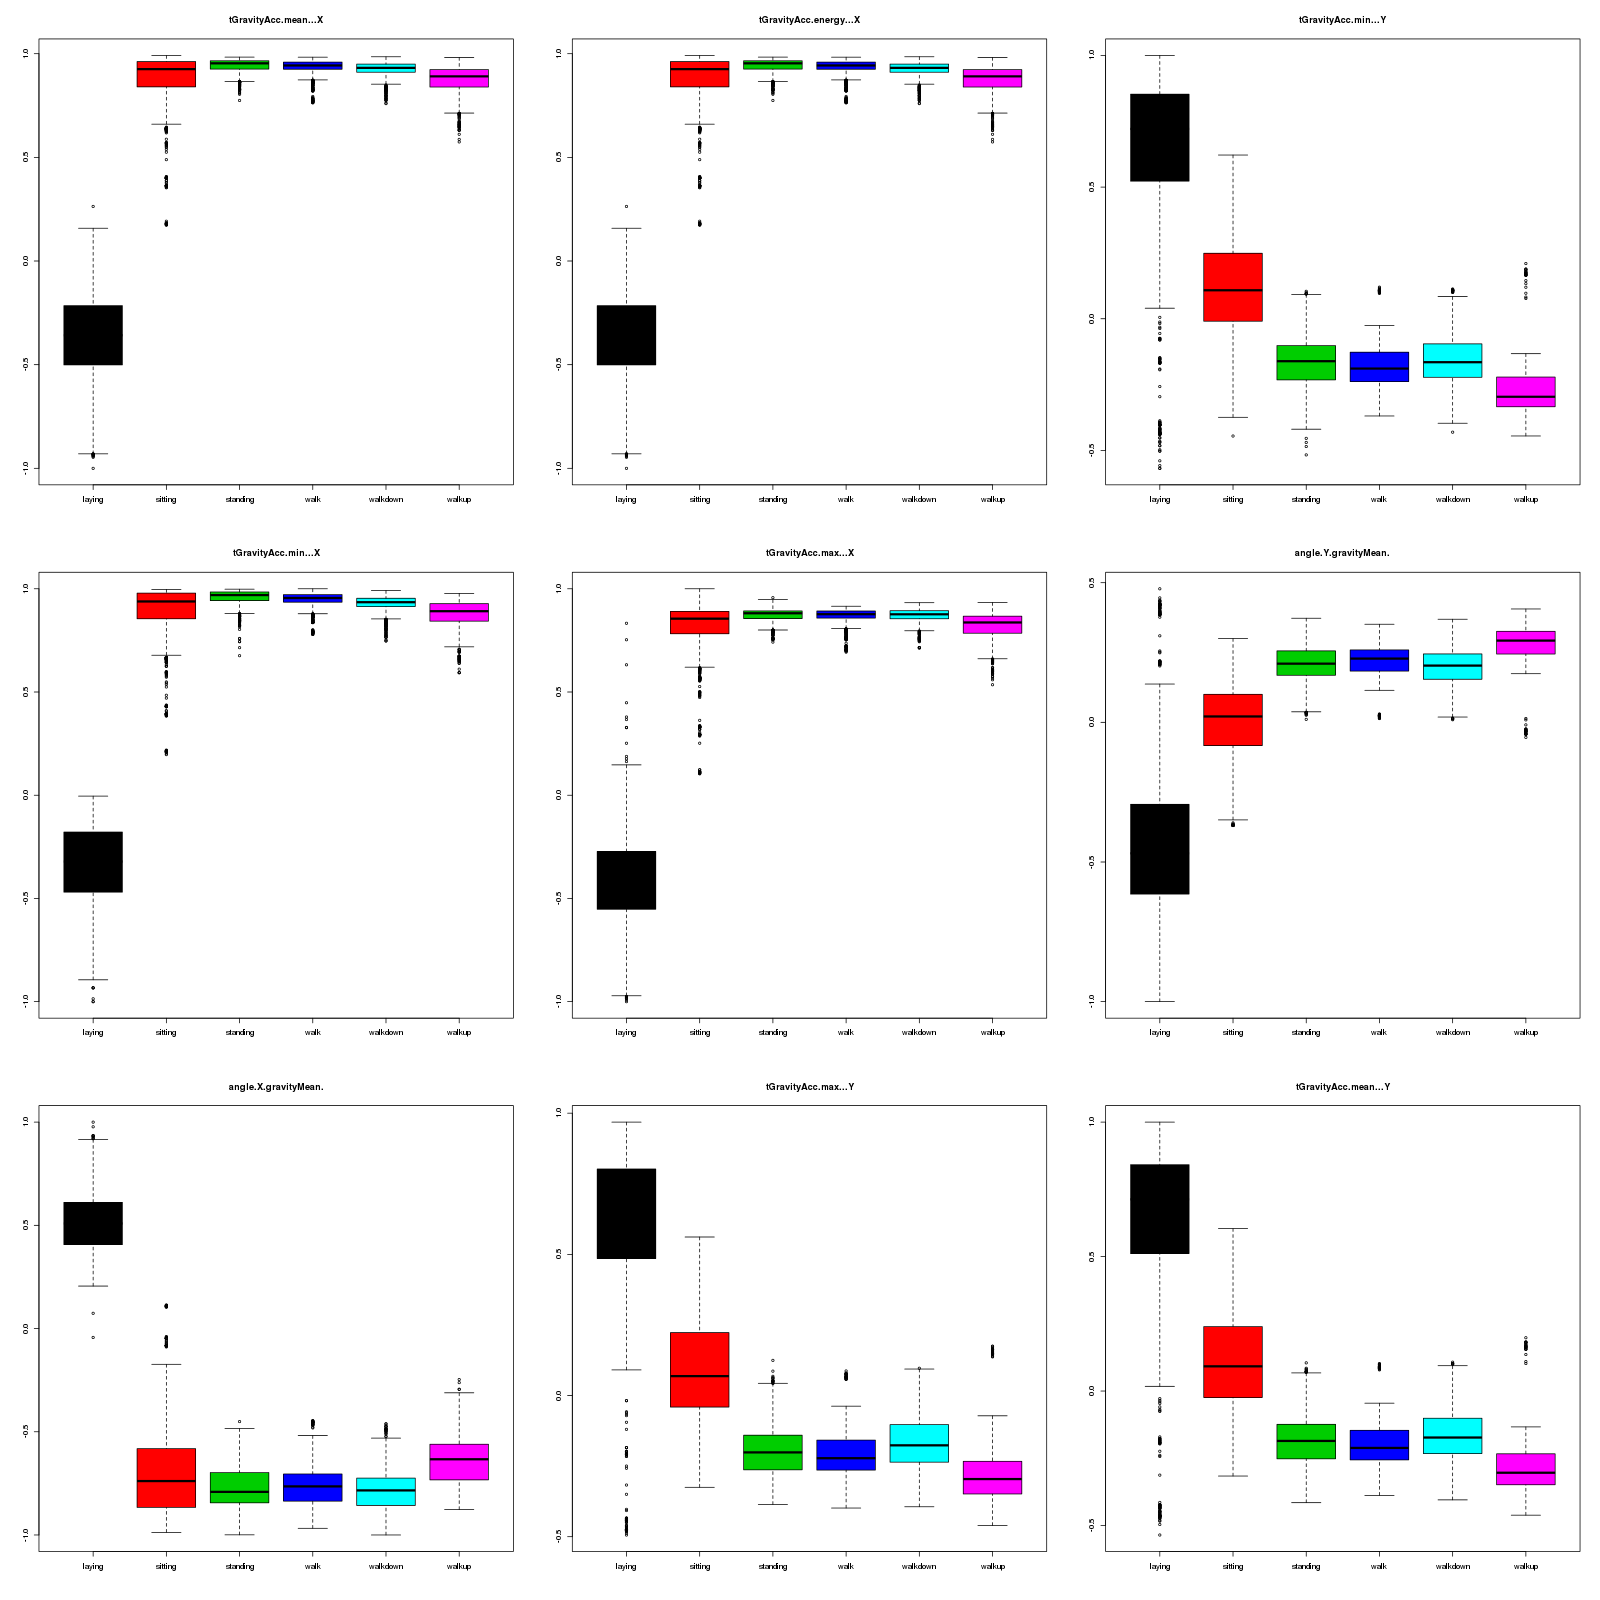
\includegraphics[width=16cm]{img/plots.png}
    \caption{}
    \label{fig:boxplots}
\end{figure}

\section{Conclusion}

As we can see, using Random Forest classifier, we built a good classifier, with
low error rates when making predictions both ing training and test sets. With
this classifier, we were also able to find the most relevant variables in
making the predictions. We could use the variables listed previously to build
another classifier avoiding overfitting. This classifier would probably be
worst in predicting in the test set, but could be even better in predicting
instances from the test set.
the training set.


\clearpage
\begin{thebibliography}{24}

\bibitem{random-forest} Random Forest package site: \url{http://www.stat.berkeley.edu/~breiman/RandomForests/cc_home.htm}
\bibitem{acelerometro} Wikipedia article about accelerometer: \url{http://en.wikipedia.org/wiki/Accelerometer}

\bibitem{murphy} Murphy-Hill, E.; Parnin, C.; Black, A. P  How we refactor, and how we know it. 
Proceedings of the 2009 IEEE 31st International Conference on Software Engineering, 2009.

\end{thebibliography}

% that's all folks
\end{document}

